\documentclass[tikz,convert={density=150,size=600,outext=.png}]{standalone}
\usetikzlibrary{shapes, calc, arrows, fit, positioning, decorations, patterns, decorations.pathreplacing, chains, snakes}
\input{../setup-web-fonts}
\input{../setup-packages}
\graphicspath{{../pictures/}} % path to pictures, trailing slash is mandatory.

% The actual drawing follows
\begin{document}
   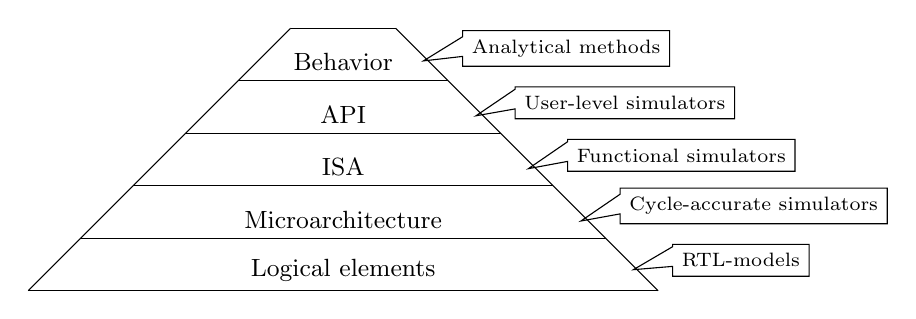
\begin{tikzpicture}
    \coordinate (A) at (-4,-4) {};
    \coordinate (B) at ( 4,-4) {};
    \coordinate (C) at ( 0, 0) {};
    \draw (A) -- ($(A)!5/6!(C)$);
    \draw (B) -- ($(B)!5/6!(C)$);
    \draw ($(A)!5/6!(C)$) -- ($(B)!5/6!(C)$);
        \foreach \y/\A/\S in {0/{Logical elements}/{RTL-models},
                            1/Microarchitecture/{Cycle-accurate simulators},
                            2/ISA/{Functional simulators},
                            3/API/{User-level simulators},
                            4/Behavior/{Analytical methods}
                            } {
            \draw ($(A)!\y/6!(C)$) -- ($(B)!\y/6!(C)$)
            node[midway,above] {\small\A}
            node[above right = 0.25cm, draw, rectangle callout, callout relative pointer={(185:0.5cm)}] {\scriptsize\S};
        }
    \end{tikzpicture}
\end{document}
